\documentclass{article}

\usepackage[danish]{babel}
\usepackage[utf8]{inputenc}
\usepackage{float}
\usepackage{fancyhdr}
\usepackage{amsmath}
\usepackage{color}
\usepackage{listings}
\usepackage{graphicx}
\usepackage{pdfpages}
\usepackage{booktabs}
%\usepackage{enumitem}
\usepackage[a4paper, top = 1in, bottom = 1in, left=1in,right=1in]{geometry}
\lstset{language=R,basicstyle=\ttfamily}

\title{Statistik og dataanalyse}
\author{Peter Heilbo Ratgen - perat17@student.sdu.dk}
\date{\today}

\begin{document}
\maketitle
\newpage
\tableofcontents
\newpage
\section{Uge 36 - Introduktion til data}
Denne uge er om kapitlet "Introduction to data".
\subsection{Introduktion til kurset}
Eksamen er en multiple choice. Undervejs er det tællende aktiviteter.

\subsection{Statistiske metoder}
Hvordan indsamler vi data, i forhold til hvad vi skal vide? Har vores data bias?
Vi har alle sammen bias på en eller anden led. Vi skal gerne lande et sted
mellem teori, viden og virkelighed. 

Generelt for man svar som man spørger. Hvis man putter urelaterede punkter ind
og laver regression, får man altid et matematisk svar, men om dette er korrekt
er ikke relateret til den matematiske model man anvender. Statistik analyse
baserer sig på normalt distribueret data, uafhængighed og stor eller lille
stikprøvestørrelse. Ved ikke at følge disse principper kan vi drage forkerte
konklusioner fra dårlig data. Den teoretisk model er korrekt nok, men vi kan
ikke drage
konklusioner fra dårlig data.

En normalfordeling er den fine lille klokkekurve, fx højde, IQ, vægt, mv. Når
man har data nok vil det blive normalfordelt. Generelt set, skal man lave være
med at arbejde i små populationer.
Data må ikke kunne påvirke hinanden, uafhængighed er det vigtigste i statisk.
Det er hele præmissen for statetisk.

\subsection{Arbejde med data}
Vi skal have en stikprøve. Vi starter med en hypotese. Så skal vi finde en model
i den statistiske værktøjskasse. Nogengange ligger svære i at finde det rigtige
værktøj. Så estimerer vi, hvad vi før ud af den model vi har valgt. Man har
selvfølgelig en forventning om hvad der skal komme ud. Derefter evaluerer vi
resultatet af modelleringen fx. har jeg fået det ud af det jeg forventede?

\subsection{Population til stikprøve}
Man skal have en stikprøve fra den samlede population. En stikprøve er korrekt
når den ikke er biased eller noget i den retning. Stikprøven skal være
repræsentativ for den samlede population. Den skal også være stokastisk, man
skal sikre sig at den man vælger, faktisk er tilfældig.
Så kan konklusion der drages af stikprøven, anvendes på den større population.

\subsection{Data}
Vi har forskellige typer af data. 

\begin{itemize}
  \item Kontinuert - numerisk
    \subitem en flydende overgang i data, fx hvor gammel nogen er. En person
    er et vidst antal år, måneder, dage, timer, sekunder, milisekunder, osv.
  \item Diskret  - numerisk
    \subitem Enkelte tal, fx en karakterrække
  \item Ordinær - kategorisk,
    \subitem Kategorisk data har en naturlig orden til sig. I bogen er givet
    eksemplet med forskellige uddannelsesniveauer, her der forskellige
    kategorier, men disse kategorier har en bestemt orden mellem sig.
  \item Nominel - kategorisk
    \subitem Nominelle variabler er kategoriske, men har ingen særlig orden til
    sig, modsat ordinære variabler.
\end{itemize}

Association er ikke det samme som kausalitet. Kausalitet kan kun drages fra
randomiserede eksperimenter. Hvis man bare kigger på tal og tænker sig til en
sammenhæng, kan man drage forkerte konklusioner. Et eksempel er Minnesota, med
bøgerne i trailerparkerne, der var blevet sat ud på grund af at man havde
fundet, det gik bedre for børn i hjem med bøger.

\subsection{Statistik og programmering}
  Vi kan bruge mange værktøjer til at lave statetisk. Vi bruger R. Python kan
  også bruges til den slags. R er lavet specifikt til formålet, det er lavet af
  statistikere.

\newpage
\section{Uge 37 - Deskriptiv statistik}
Deskriptiv statistik er en måde at bearbejde data på, med visualisering og
nøgletal, som fx varians. Det handler om, hvad kan vi sige om de her tal.

\subsection{Metode}
\begin{itemize}
  \item Histogram
  \item Beregninger
  \item Konfidensinterval
  \item Box-plot og undersøgelser af ekstremer
\end{itemize}

Vi skal ud af en deskriptiv analyse finde, hvad der er typisk. Hvor symmerisk er
datasættet, hvad er det der afviger fra det man ville forvente, lidt til den ene
eller anden side i en fordeling af karakterer. Koncentrationen af datasættet,
mange vil få 4 eller 7, og få vil få 12. Igen, hvad må vi forvente? Er der nogle
ekstremer i datasættet? 

\subsection{Histogram}
Man bruger ca. 8 til 12 kolonner på data. Med mindre der er andet der giver
mening. Vi grupperer kun data, hvis det giver mening. Selv hvis vi har en
terning med 100 sider, selvom det man får ud er diskret, kan man godt gruppere
det data. 
Når en kurve har en hale til venstre, så er den venstreskæv.


Vi kan lave et histogram i R.

\begin{lstlisting}
eksempel <- rnorm(200, mean = 50, sd = 15)
hist(eksempel, main = "Whats the topic",
  xlab="name of the variable its",
  xlim=c(20,90),
  col="blue")
\end{lstlisting}

\subsection{Positionsmål}

\begin{itemize}
  \item Gennemsnit
    \subitem $$\frac{x_1+x_2+x_3+\dots + x_n}{n}$$
  \item Modus eller modal?
    \subitem Den prøve eller prøver der forekommer flest gange. Vi tæller de
    toppe der forekommer flest gange. Man kan have unimodus, bimodus og
    multimodus.
  \item Median
    \subitem Midten af et datasæt, det er ikke det samme som et gennemsnit.
  \item 5-punkts opsummering, kvartiler, deciler
\end{itemize}

\subsection{Variansmål}

\begin{itemize}
  \item Varians
    \subitem $$\frac{\sum^{n}_{i=1}x_i - \bar{x}}{n-1}$$
  \item Standardafvigelse
    \subitem $$\frac{\sum^{n}_{i=1}x_i - \bar{x}}{n-1}$$
  \item Normaliseret varians (Standard error) 
  \item Varianskoefficient
  \item Inter kvartil interval 
    \subitem $Q_3 - Q_1$
  \item Inter decil interval 
    \subitem $D_9-D_1$
  \item Skævhed
    \subitem Symmetri
  \item Kurtose
    \subitem Densitet eller koncentration. Ved en høj værdi er data meget tæt.
\end{itemize}

\subsection{Box-plot}
Med en boxplot kan vi identificere outliers. En outlier er mere end 3 gange IRQ
væk fra $Q_3$ eller $Q_1$ (inter quartile range). En mistænkt outlier er 1.5 gange IRQ
væk fra $Q_3$ eller $Q_1$.
Man må ikke bare smide en outlier væk, uden af tænke over hvorfor man vil smide
det ud af datasættet. Vi laver et boxplot med

\begin{lstlisting}[escapeinside={(*}{*)}]
boxplot(airquality(*\$*)Ozone,
  main = "Some title",
  xlab = "x label",
  ylab = "y label",
  col = "orange",
  horizontal = TRUE
  )
\end{lstlisting}

\subsection{Grupperede datasæt}
Hvis vi laver at histogram i kontinuert data, kan søjlerne røre hinanden. Hvis
vi laver det med diskret data, skal der gerne være et mellemrum mellem søjlerne.
Underviseren kan dog ikke finde ud af det selv.

\subsection{Konfidensinterval}
Det handler om en stikprøve har et gennemsnit, den stikprøve er
    taget i en population hvis gennemsnit er $\mu$, hvis vi laver en stikprøve
    hvis gennemsnit er $\bar{x_1}$, en anden stikprøve har gennemsnittet
    $\bar{x_2}$ og en tredje har gennemsnit $\bar{x_3}$. Gennemsnittet er så 
    $$\mu = \bar{x} \pm 1.96 - \frac{sd}{\sqrt{n}}  $$ Her er $sd$ standard
    afvigelsen.
    
    \newpage
\section{Uge 38 - Sandsynlighed}
\subsection{Hvad er en sandsynlighed}
Sandsynlighed er hvad er andelen af gange, som udfaldet hænder, hvis vi
observerer en vilkårlig proces et uendeligt antal gange. Sandsynlighed  er altid
mellem 0 og 1. For diskrete udfald:
$$\sum^U_{i=1} P(x_i) = 1 $$
For kontinuerte udfald:
$$\int^{\infty}_{-\infty} P(x_i) = 1 $$

Når antallet af kast går mod uendeligt, så vil $\hat{p}(x)$ gå mod
sandsynligheden $P(x)$. Eller $\lim_{n\rightarrow \infty} \hat{p}(x) = P(x)$.
Dette kalder vi for Store Tals Lov. 

\paragraph{Disjunkte udfald}
Disjunkte udfald er uafhængige af hinanden. Så ligemeget hvor mange gange man
kaster en terning har det ikke nogen indflyelse på de andre terningekast. Vi kan
lægge sansynlighederne for disse hændelser sammen:

$$P(A_1 \ \text{eller} \ A_2) = A_1 + A_2$$

Så hvis vi har $k$ udfald der er disjunkte, da kan vi:
$$P(A_1 \ \text{eller} \ A_2 \ \text{eller} \ \dots \ \text{eller} \ A_k) = P(A_1) + P(A_2) + \dots + P(A_k)$$
\paragraph{Ikke-disjunkte udfald}
Hvis vi kigger ikke-disjunkte udfald, altså hvor forskellige sandsynligheder
påvirker hinanden. Vi må ikke tælle de samme ting to gange, så vi trækker det
der overlapper fra. Et eksempel er et kortspil, hvor vi har to hændelser $A$:
ruder og $B$: billedkort. Her er sandsynlighederne: $$P(A)=\frac{13}{52} =
\frac{1}{4}$$ $$P(B) = \frac{12}{52} = \frac{3}{13}$$. Da begivenhederne ikke er
uafhængige kan vi ikke bare: $\frac{13}{52} + \frac{12}{52} = \frac{25}{52}$.
Dette er da vi tæller rudernes billedkort med to gange. Vi skal finde
fællesmængden, denne skrives som: $P(A \cap B) = \frac{3}{52}$. Denne skal du
trækkes fra. 
$$P(A) + P(B) - P(A\cap B) = \frac{13}{52} + \frac{12}{52} - \frac{3}{52} =
\frac{13+12-3}{52}=\frac{22}{52} = \frac{11}{26}$$

\paragraph{Sandsynlighedsfordelinger}
En sandsynlighedsfordeling er en tabel med alle disjunkte udfald og deres
tilhørende sandsynligheder. Reglerne for en sandsynlighedsfordeling er at:
\begin{itemize}
  \item Udfaldet, som skal være disjunkt skal kunne listes
  \item Hvor sandsynlighed må ligge mellem 0 og 1
  \item Summen af sandsynlighederne må være 1
\end{itemize}

\paragraph{Komplementærmægde}
Vi har det samlede udfaldsrum $U = \{1, 2, 3,4,5,6\}$.  Vi definerer en hændelse
D, som viser øjnene $D = \{2,3\}$. Dennes komplementærmængde er: $D^{C} =
\{1,4,5,6\}$. Hvis vi har en sandsynlighed $P(D) = \frac{1}{3}$, da er
komplementærmængden $$P(D^C) = 1 - P(D) = 1 - \frac{1}{3} = \frac{2}{3}$$

\paragraph{Uafhængige hændelser}
Ved uafhængige hændelser påvirker sandsynlighederne for hændelse 1 og 2 ikke
hinanden. Fx påvirker to terningekast ikke hinanden. Hvis vi tre terninger, en
rød, blå og hvid. Sandsynligheden for at alle tre terninger viser 6 er:
$$P(\text{rød terning} \ =6)P(\text{blå terning} \ =6)P(\text{hvid terning} \
=6) = \frac{1}{6}\cdot \frac{1}{6} \cdot\frac{1}{6}$$.
En generel regel er:
$$P(A_1 \cap A_2 \cap \dots \cap A_k = P(A_1) \cdot P(A_2) \cdot \dots \cdot
P(A_k) $$

\paragraph{Marginale sandsynligheder}.

\begin{table}[h]
  \centering
  \begin{tabular}{l|l|l|l|l}
   &                    & Sandt  &           &        \\\hline
   &                                       & Mode   & Ikke mode & Total  \\\hline
   machine\_learning & Forudsigelse\_mode & 197 & 22    & 219 \\\hline
   & Forudsigelse\_nej  & 112 & 1491    & 1603 \\\hline
   & Total              & 309 & 1513    & 1822   
  \end{tabular}
\end{table}

Sandsynligheder

\begin{table}[H]
  \centering
  \begin{tabular}{l|l|l|l|l}
   &                    & Sandt  &           &        \\\hline
   &                                       & Mode   & Ikke mode & Total  \\\hline
   machine\_learning & mode & 0.1081 & 0.0121    & 0.1202 \\\hline
   & nej  & 0.0615 & 0.8183    & 0.8798 \\\hline
   & Total              & 0.1696 & 0.8304    & 1.0   
  \end{tabular}
\end{table}

\subsection{Betinget sandsynlighed}
Vi finder sandsynligheden for at det er mode givet at machine-learning har sagt
at det er mode.

$$P(\text{mode givet machine\_learning.mode}) = \frac{197}{219} = 0.9$$
$$P(\text{mode $|$ machine\_learning.mode}) = \frac{197}{219} = 0.9$$

Vi kan se at det er det samme som:
$$P(\text{mode $|$ machine\_learning.mode}) = \frac{197}{219} =
\frac{\frac{197}{1822}}{\frac{219}{1822}} = \frac{P(\text{mode $\cap$
machine\_learning.mode})}{P(\text{machine\_learning.mode})} $$

Mere generelt kan vi skrive at sandsynligheden for A givet B skrives ved:
$$P (A \bar B) = \frac{P( A \cup B)}{P(B)}$$ Vi skal huske at vi skal dele med
sandsynligheden for betingelsen. Hvis de er uafhængige da ved vi
$$P(A \cap B) = P(A) \cdot P(B) $$

$$P(A \bar B) = \frac{P(A\cap B)}{P(B)} = \frac{P(A) \cdot P(B)}{P(B)} = P(A)$$

\newpage
\section{Uge 39 - Fordelinger \\ Fordelinger for stokastiske variable} 

\subsection{Diskrete fordelinger}
\paragraph{Den hypergeometriske fordeling}
En diskret fordeling, vores population består af $s$ successer og $N-s$
fiaskoer. Vi udtrækker vores stikprøve $(n)$ fra en endelig population $(N)$
Vores stikprøve består af $x$ succeser og $n-x$ fiaskoer Vi benytter uden
tilbagelægning Fordelingen kræver følgende parametre: $N, n, m$.


Den hypergeometriske fordeling kan approksimeres til binomialfordelingen, når
poppopulationen $N$ er stor, og stikprøven $n$ er lille. Dette brugtes forhen,
før man brugte computere.

\paragraph{Geometriske fordeling}
Den stokastiske variable $X$ er Bernouli fordelt, idet vi har to udfald. Enten
har vi succes, med sandsynligheden $p$, eller fiasko, med sandsynligheden $1-p$.
$p$ estimereres med:

$$\hat{p} = \frac{\text{antal succeser}}{\text{antal forsøg}}$$

For at kunne anvende dette (Bernouli fordelingen). Skal være $n$ forsøg, der kan
kune være to udfald, det kræver at man har samme sandsynlighed hver gang og at
der skal være uafhængighed. 

Den geometriske fordeling er eksponentielt aftagende.
\paragraph{Binomialfordelingen}
Vi deler i succes $p$ og fiasko $1-p$. Vi udtrækker vores stikprøve (n) fra en
endelig population (N) med tilbagelægning.


\paragraph{Negativ binomialfordeling}
\paragraph{Poissonfordelingen}

\subsection{Kontinuerte fordelinger}
\paragraph{Uniformfordeling}
\paragraph{Normalfordeling}
\paragraph{t – fordeling}
\paragraph{F – fordeling}
\paragraph{$x^2$  - fordeling}

\newpage

\section{Uge 40 - Konfidens og p-tests}

\section{Uge 41 - Tests II}



\section{Øvelser - Uge 37}
\subsection{Opgave 1}
Præsentationen af et normalfordelt datasæt med 500 observationer. En middelværdi
på 70 og en standardafvigelse 15.
\begin{figure}[H] 
  \centering
  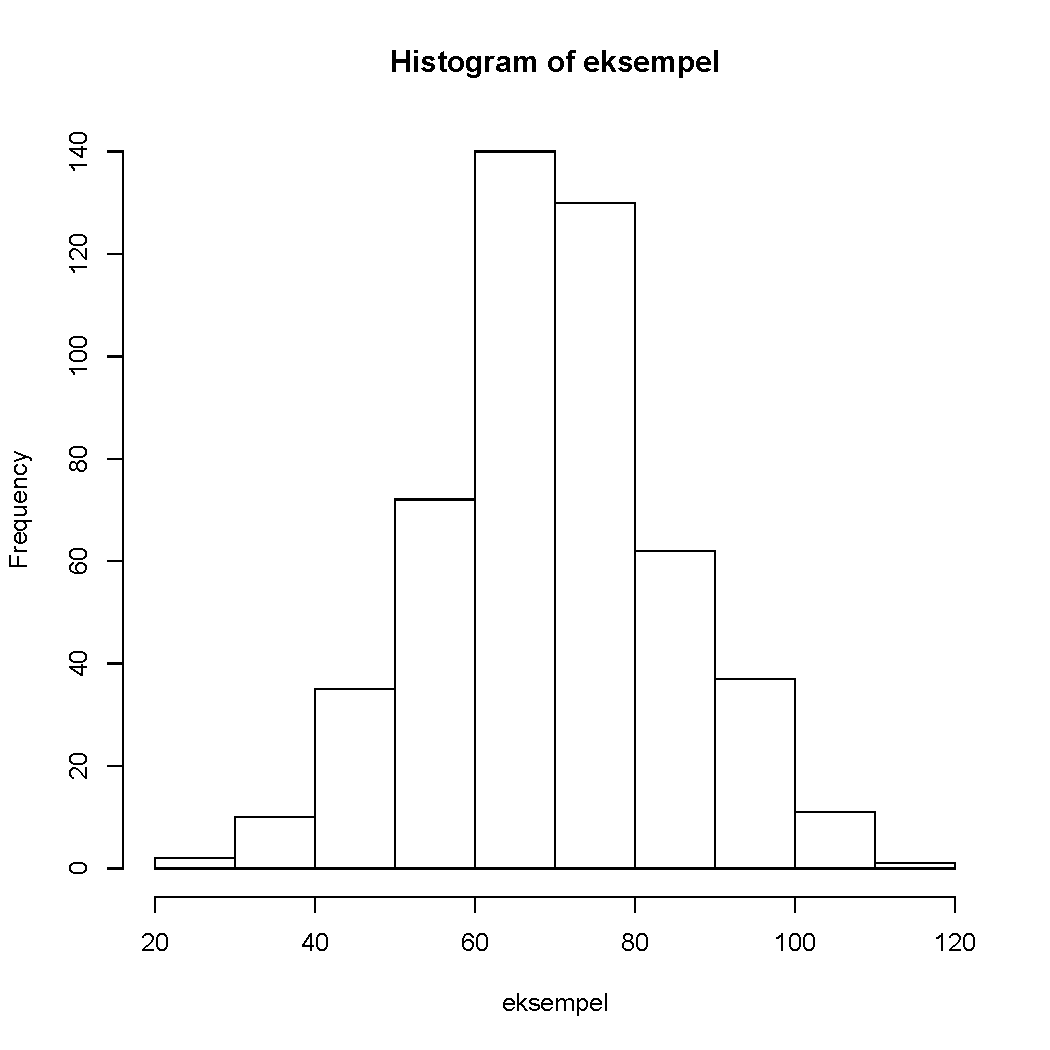
\includegraphics[width=0.5\textwidth]{../velser/uge37/R/opg1.pdf}
\end{figure}

\subsection{Opgave 2}
Vi har sat vores datasæt ind i R. Vi skal lave en beskrivende statetisk. Den
beskrivende statistik går ud på:
\begin{itemize}
  \item Opsætning af et histogram eller en tidsserie.
  \item Udregning af beskrivende statetiskker.
  \item Opsætning af et konfidensinterval
  \item Opsætning af et boxplot og undersøgelse af eventuelle outliers.
\end{itemize}

\paragraph{Tidsserie} Dette en tidsserie over antal kunder i butikken.

\begin{figure}[H] 
  \centering
  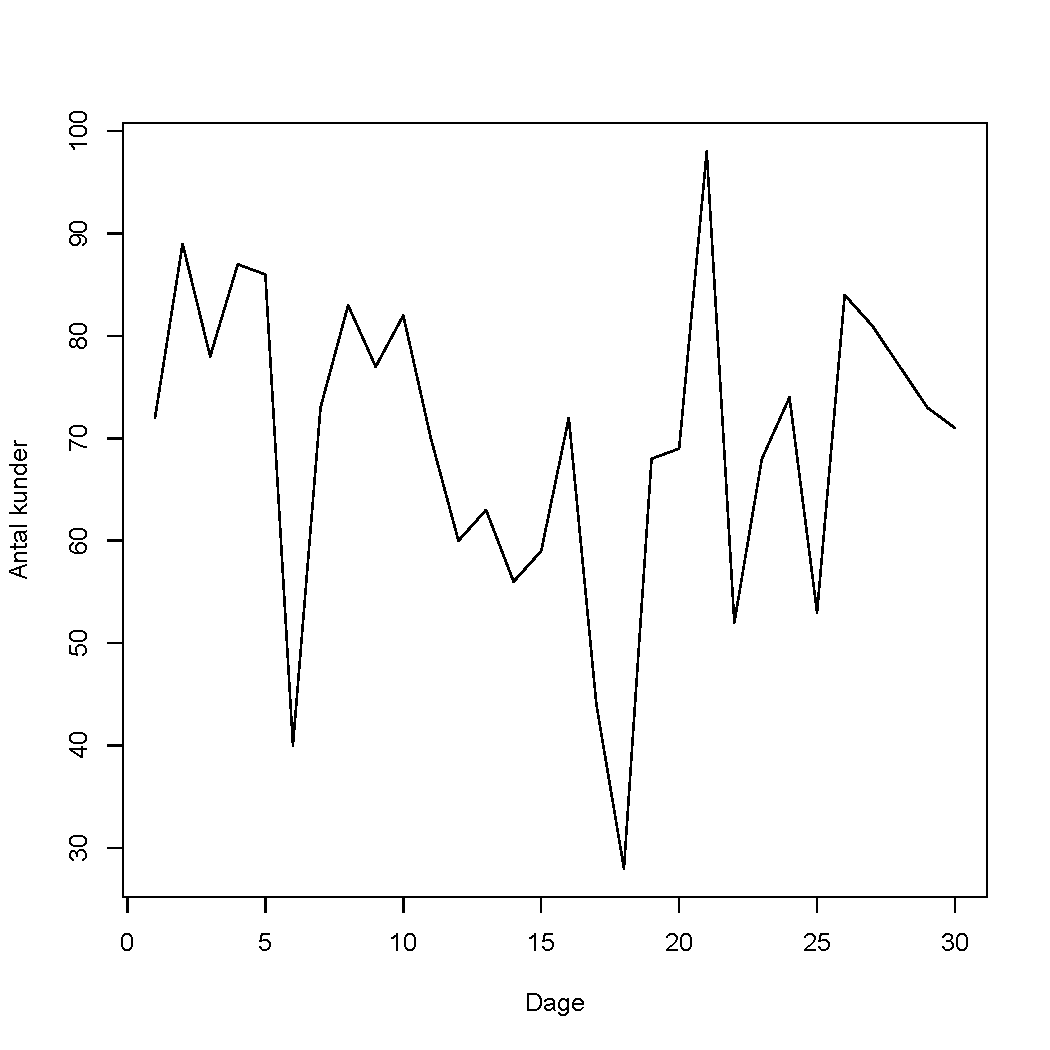
\includegraphics[width=0.5\textwidth]{../velser/uge37/R/opg2.pdf}
\end{figure}
Tidsserien viser at antallet af kunder per dag. Dette viser at antallet af
kunder svinger meget fra dag til dag.

\paragraph{Beskrivende statetiskker}


\end{document}
